\documentclass[a4paper,landscape,titlepage,17pt]{extarticle}
\usepackage{color,amsmath,graphicx}
\usepackage[citestyle=numeric,backend=bibtex]{biblatex}
\usepackage[labelfont=bf]{caption}
\usepackage[affil-it]{authblk}
\usepackage{fullpage}
\usepackage{pdflscape}
\linespread{1}
\pagenumbering{gobble}
\bibliography{library}

\title{\Huge Increased concentration of proteins with growth rate can result from passive resource redistribution}
\author{\Large Uri Barenholz, Leeat Keren, Ron Milo}
\affil{The Weizmann Institute of Science, Rehovot, Israel}
\date{}

\begin{document}
\maketitle
\section*{\LARGE Abstract}
In many microorganisms, the proteome composition changes dramatically as a function of the growth environment.
Furthermore, many of these changes seem to be coordinated with the growth rate rather than the specific environment.
However, although cellular growth rates, gene expression levels and gene regulation have been at the center of biological research for decades, their quantitative interdependence is not yet fully understood.

We analyzed the relationship between growth rate and proteome composition for the model microorganism \emph{E.coli} as reflected in two proteomics data sets spanning various growth conditions.
We found that the cellular concentration of a large fraction of the proteins measured coordinately increases with the growth rate.
This fraction includes proteins spanning different functional groups and proteins that are involved in different cellular processes.
Notably, Ribosomal proteins are only a small fraction of this group of proteins.

We present a simple model that demonstrates how such a widely coordinated increase in the concentration of many proteins can be the result of passive redistribution of resources, due to active regulation of a few proteins.
Our model provides a potential explanation for why and how such changes relate to the growth rate under different environmental conditions.
The model thus suggests that, although the concentrations of many proteins change with the growth rate, such changes could be part of a global effect, not requiring specific cellular control mechanisms.
\clearpage        
\section*{\LARGE Results}
\subsection*{Many proteins are positively correlated with growth rate}
The Pearson correlation between the concentration of every protein and the growth rate in the two data sets (denoted by V for data from \parencite{Valgepea2013} and by H for unpublished data from M. Heinemann's lab) is shown in Figure \ref{fig:growthcorr}.
The two data sets present a large number of proteins ($724$ out of $1981$ measured in H and $296$ out of $2184$ in V) that are significantly positively correlated with the growth rate \footnote{High correlation proteins are defined as those with a Pearson correlation in the range $(0.4,0.8)$ and $(0.8,1)$ for the H and V data sets, respectively}.
Notably, the proteins that present high correlation with the growth rate are involved in different cellular functions and span different functional groups.

The lower correlation and higher variability found in the H data set may result from the fact that it contains much more conditions but spans roughly the same range of growth rates.
Furthermore, it includes measurements of the proteome under conditions involving different carbon sources as opposed to the V data set that uses the same carbon source in all measurements.
This is exemplified by restricting the analysis of the H data set only to chemostat conditions (Figure \ref{fig:growthcorrchemo}).

\begin{figure}[h]
\centering
\includegraphics[scale=1.9]{GrowthRateCorrelation.pdf}
\caption{\linespread{0.5}\selectfont{}
A significant fraction of the proteins have positive correlation with the growth rate in the two data sets analyzed.
These proteins span many functional groups.
Proteins with unknown function (present in the Heinemann data set, right panel) show less correlation with growth rate, as well as proteins with low levels of expression (data not shown).
}
\label{fig:growthcorr}
\end{figure}

\clearpage        
\subsection*{Proteins that are positively correlated with growth rate share a similar, significant response}
We examined how large is the response of the proteins that have a significant positive correlation with the growth rate across the conditions measured (referred to as high correlation proteins).
To this end, we summed up the concentrations of all of the high correlation proteins across the conditions measured and compared their total concentration to the growth rate (Figure \ref{fig:globalgrcorr}).
Both data sets presented a significant response ($\approx 2$ fold change in total concentration across $\approx 5$ fold change of the growth rate) with most of the variability of the total concentration being explained by the growth rate ($R^2$ of $0.75$ in H and $0.99$ in V). 

We note that two proteins that have equal, non-perfect, correlation with the growth rate may not be correlated between themselves.
Furthermore, they may scale differently with the growth rate.
To test whether the high correlation proteins indeed share a common response, we normalized the concentration of every such protein across the conditions measured to 1, and then calculated the slope of a linear regression line with the growth rate for that protein.
This analysis revealed that most proteins respond in a similar manner across the different growth conditions (Figure \ref{fig:globalfit}).

\subsection*{Ribosomal proteins share the same response to growth rate as other proteins}
We examined how the response of high correlation proteins relates to the well-studied response of the ribosomal proteins.
We therefore performed the same analysis of slopes, restricting it to ribosomal proteins alone (Figure \ref{fig:globalfit}).
The analysis shows that, on average, high correlation proteins scale in the same way as ribosomal proteins do.
\clearpage        

\begin{figure}[h]
\centering
\includegraphics[scale=1.7]{GlobalClusterGRFit.pdf}
\caption{\linespread{0.5}\selectfont{}
The sum of the concentrations (as fractions out of the proteome) of high correlation proteins in each of the data sets, with linear regression lines, is shown.
High correlation proteins form a large fraction out of the proteome at higher growth rates ($>40\%$ for H and $>50\%$ for V).
The change in the total concentration of high correlation proteins is about 2-fold while the growth rate changes by about 5-fold.
Some of the unexplained variability of high correlation proteins in the H data set can indicate errors in growth rate measurements and/or differences in degradation rates across conditions.
(High correlation proteins are defined as those with a Pearson correlation in the range $(0.4,0.8)$ and $(0.8,1)$ for the H and V data sets, respectively)
}

\label{fig:globalgrcorr}
\end{figure}
\clearpage        
\begin{figure}[h]
\centering
\includegraphics[scale=1.9]{AllProtsVSRibosomalNormalizedSlopes.pdf}
\caption{\linespread{0.5}\selectfont{}
    A histogram of the normalized slopes of the trend lines for every high correlation protein (blue), and for every ribosomal protein (green) is shown for the two data sets analyzed.
    Left panel - data from \parencite{Valgepea2013}, right panel - data from the Heinemann lab.
    High correlation proteins all share a relatively similar response, meaning they maintain their relative ratios.
    Ribosomal proteins respond in a similar manner to the rest of the high correlation proteins .
}
\label{fig:globalfit}
\end{figure}
\clearpage        

\begin{figure}[h]
\centering
\includegraphics[scale=1.9]{HeinmannChemostatGr.pdf}
\caption{\linespread{0.5}\selectfont{}
  Restricting the analysis of the Heinemann data set to chemostat conditions yields similar results to those obtained for the Valgepea data set.
}
\label{fig:growthcorrchemo}
\end{figure}
\clearpage        

\subsection*{Theoretical model}
In an attempt to explain how such a wide-span positive response occurs, we have constructed a minimalistic model that is able to reproduce these results as the outcome of redistribution of resources of the bio-synthesis machinery.
Briefly, the model assumes that favorable growth conditions allow the cell to down-regulate some proteins that are needed in harsher conditions, thus reducing the amount of proteins that need to be produced for the cell to proliferate (Figure \ref{fig:model}).
As a consequence, the fraction of each of the rest of the proteins out of the proteome increases, assuming they are being expressed in the same relative ratios.
The growth rate therefore increases as well, due to the fact that the ratio of bio-synthetic machinery to the rest of the proteome increases.

According to the model, for non-differentially regulated proteins, their concentration should drop to 0 when the growth rate is 0.
Interestingly, protein degradation affects the expected concentration of non-differentially regulated proteins at 0 growth rate.

Assuming that protein degradation acts on all proteins in the same way, and that it is invariant in the growth rate, the effect of protein degradation can be understood as follows: at any time, some fraction of the entire proteome is degraded.
Therefore, the \emph{observed} growth rate, $\mu$, is, in fact, equivalent to the amount of proteins produced minus the amount of proteins degraded.
To illustrate, if the measured growth rate is 0, the implication is not that no proteins are produced, but rather that proteins are produced at exactly the same rate as they are degraded.
\clearpage
\begin{landscape}
\begin{figure}[h]
\centering
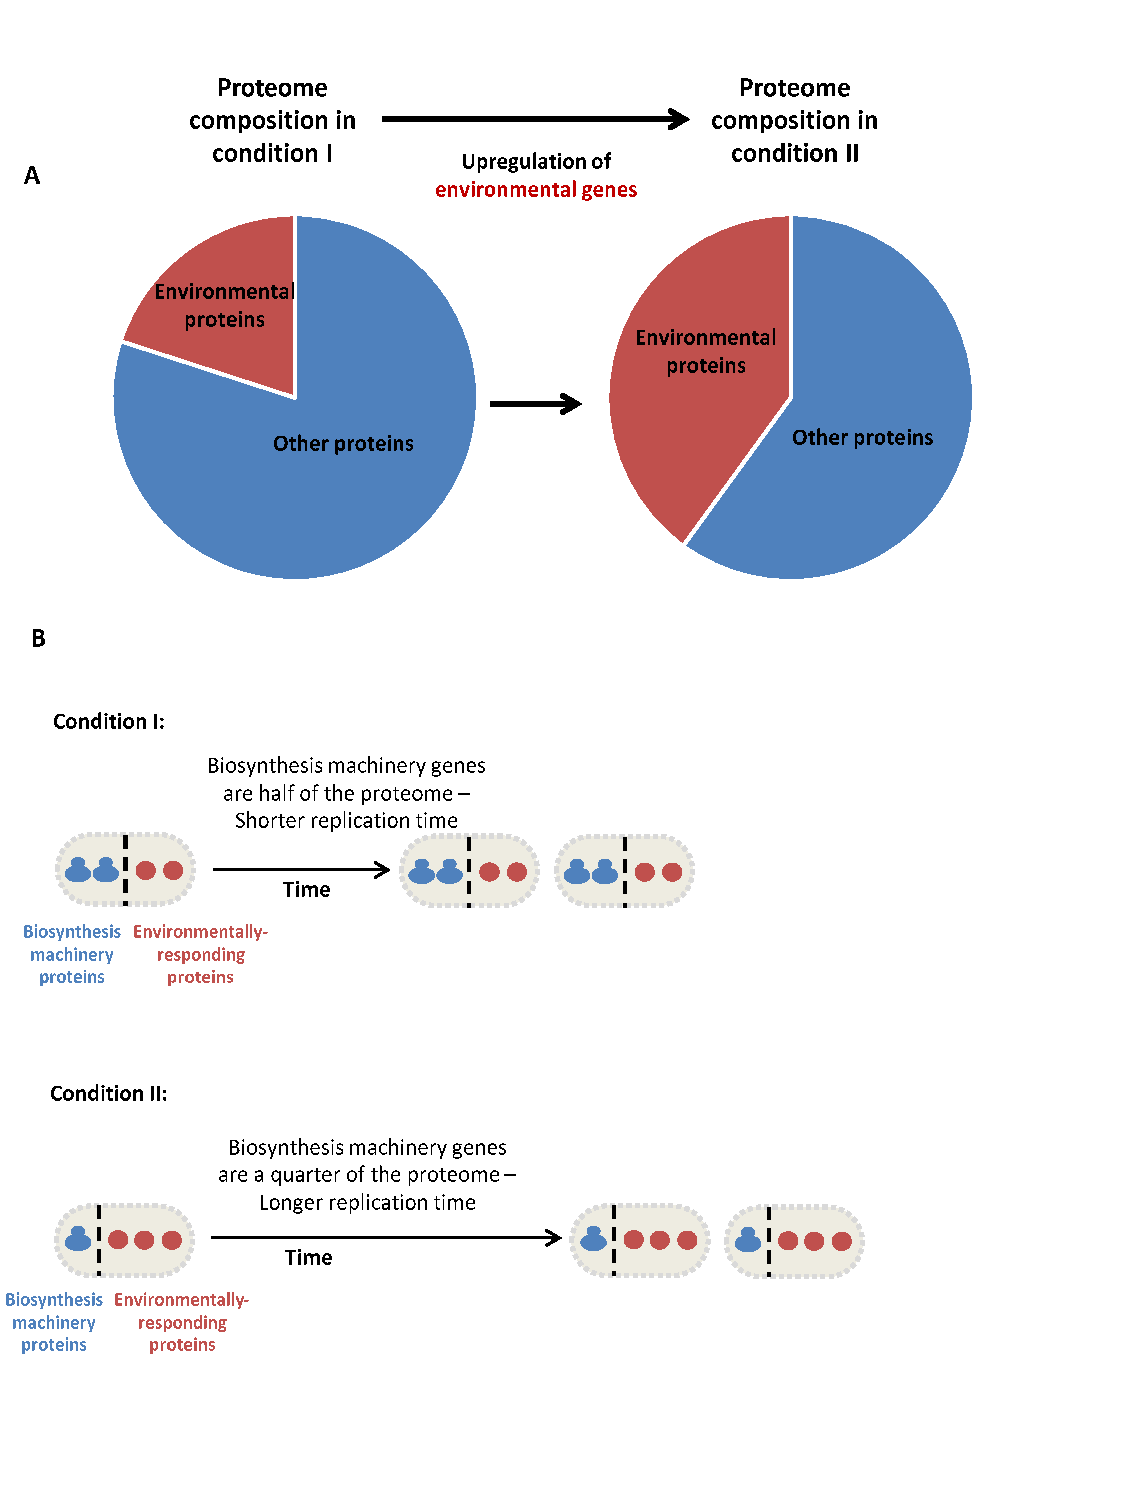
\includegraphics[scale=0.9]{Figures7-trieste.pdf}
\caption{\linespread{0.5}\selectfont{}
  A minimalistic model predicts up regulation of environmental genes reduces the concentration of other proteins (Panel A).
As a result, the ratio of bio-synthesis machinery genes to the rest of the proteome decreases, resulting in slower growth (Panel B).
}
\label{fig:model}
\end{figure}
\end{landscape}
\clearpage        


\printbibliography
\end{document}